% !TEX encoding = UTF-8 Unicode
\documentclass[12pt, a4paper]{article}
\usepackage[ngerman]{babel}
\usepackage[utf8]{inputenc}
\usepackage[T1]{fontenc}
\usepackage{lmodern}
\usepackage{graphicx}
\usepackage{epstopdf}
\usepackage[margin=1in]{geometry}
\usepackage{titling}
\usepackage{hyperref}
\usepackage{amsmath}
\usepackage{braket}
\usepackage[expproduct=\cdot]{siunitx}
\usepackage{mhchem}
\AtBeginDocument{\sisetup{math-rm=\mathrm, text-rm=\rmfamily}}
\renewcommand{\familydefault}{\sfdefault}
\setlength{\droptitle}{-2cm}
\title{Auswertung zu IQ13:\\
       magneto-optische Falle\\
       WiSe 15/16\\
       Block III}
\author{Ramin Javadi 2993630 und Felix Schrader 3053850}
\date{}
\begin{document}
\maketitle
\tableofcontents
\newpage
\section{Theorie einer magneto-optischen Falle}
  \subsection{Optische Melasse}
  Laserkühlung von Atomen, das ist die Reduktion der atomaren Geschwindigkeitsverteilung, in diesem Fall durch Laserlicht. Dabei spielt der Strahlungsdruck wichtige Rolle, der zur Spontankraft führt. In einer Dimension betrachten wir die Wechselwirkung eines Lasers mit einem Zwei-Niveau-Atom mit der Übergangsfrequenz ${\omega_A}$. Wenn ein Laser gegenüber ${\omega_A}$ rotverstimmt ist und ein entgegenkommendes Atom eine Geschwindigkeit ${\vec v}$ hat, wird dieses Atom aufgrund des Dopplereffekts Photonen absorbieren. Danach werden von dem Atom Photonen spontan und somit ohne Vorzugsrichtung emittiert.
  
  Bei jedem Absorptions- und Emissionsprozeß findet ein Impulsübertrag statt. Wenn die Absorption aus einer Richtung passiert, ist die spontane Emission ungerichtet und auch die Impulsänderung durch sie im Mittel null. Deswegen wird ein Gesamtimpuls in Richtung des Laserstrahles auf das Atom übertragen.
 \\Auf das Atom wirkt durch die Absorption eine Kraft, sie lässt sich als Produkt aus Impulsübertrag $\hbar\vec{k}$ und der Streurate $\Gamma$ der Photonen ausdrücken: 
   \begin{align*}
  \vec F=\hbar \vec k \Gamma
  \end{align*}
  Diese Spontankraft bewirkt das Abbremsen (Kühlen) von Atomen. Wenn man die Intensität des Lasers ${I}$ erhöht, wird die Streurate größer. Sie hängt auch von der Verstimmung des Lasers ${\delta_L}$ ab. Dabei entspricht ${\Gamma =1/ \tau}$, wobei ${\tau}$ die Lebensdauer des angeregten Zustands ist.
  \\Diese Verstimmung ist die Differenz der Frequenz des Lasers ${\omega_L}$ und der atomaren Übergangsfrequenz ${\omega_A}$. Sie sollte so groß wie die Dopplerverstimmung ${\vec k \vec v}$ sein.
   \begin{align*}
    \vec F=\frac{\hbar \vec k}{2 \tau} \frac{I/I_0}{1+I/I_0+(\frac{ \delta _L-\vec k \vec v}{\Gamma /2})^2}
  \end{align*}
  Wie in Abbildung \ref{fvonv} zu sehen, wirkt bei Ausbreitungsrichtung des Atoms in $-z$-Richtung eine positive Kraft, bei Ausbreitung in $+z$-Richtung eine negative Kraft. In beiden Fällen werden die Atome auf eine Geschwindigkeit ${v\approx 0}$ abgebremst. Eine Geschwindigkeitsdämpfung ist im Bereich, wo die Kraft auf ein Atom sich linear ändert, möglich.
   \begin{figure}[h!]
  \centering
  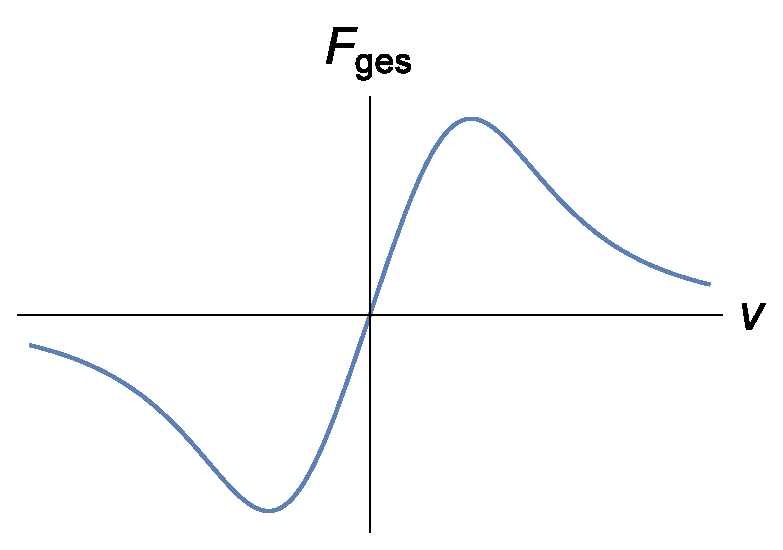
\includegraphics[width=0.5\textwidth]{fvonv.eps}
  \caption{F von v}
  \label{fvonv}
  \end{figure}
  \newpage
  Unter einer optischen Melasse versteht man diese Geometrie in drei Dimensionen. Dies erreicht man, indem drei senkrecht zueinander stehende Laser, die jeweils in sich zurückreflektiert werden. Dadurch bewirken sie die Kühlung von Atomen.
 \\In einer optische Melasse ist die Temperatur ${T}$ gegeben durch das Gleichgewicht zwischen der Kühlrate durch Absorption und der Heizrate durch den stochastischen Charakter der Emissionen.
 \\Durch die optische Melasse werden die Atome im Impulsraum gefangen. Eine Einschränkung im Ortsraum ist alleine damit jedoch nicht möglich, deswegen ist eine optische Melasse ist keine echte Falle.
 
 Durch ein zusätzliches Quadrupol-Magnetfeld kann eine Einschränkung im Ortsraum erreicht werden. Dies ist die Grundlage für die magneto-optische Falle (engl. magneto-optical trap (MOT)).
\subsection{Magnetfeld}
 Wir betrachten wieder ein Zwei-Niveau-Atom mit einem Grundzustand $\ket{J=0}$ und einem angeregten Zustand $\ket{J=1}$. 
  \\Man erzeugt ein Quadrupol-Magnetfeld ${\vec B}$, um eine Ortsabhängigkeit der Resonanzfrequenz ${\omega_0}$ zu erhalten. Wegen Zeeman-Effekts wird der angeregte Zustand aufgespalten in drei Zustände ${m_J=-1,0,1}$.
  
  Es werden zwei zirkular polarisierte und bzgl. $\omega_0$ rotverstimmte Laser entgegengesetzt auf die Atome eingestrahlt. Der rechte Laser ist linkszirkular polarisiert und der linke Laser rechtszirkular polarisiert.
  \\Solange ein Atom sich nicht bewegt, wirkt keine Kraft. Bewegt sich ein Atom z.B. nach links vom Zentrum der Falle weg, so absorbiert es mit hoher Wahrscheinlichkeit ein Photon aus dem ${\sigma^+}$-Strahl, weil es mit diesem rotverstimmten Laser in Resonanz kommt. Das Atom wird in den Zustand $\ket{J=1 , m_J=+1}$ angeregt und gekühlt. Analog wird ein Atom nach links zurückgetrieben, wenn es sich nach rechts aus dem Fallenzentrum bewegt. 

  Es wird also auf die Atome eine Kraft ausgeübt, die dazu führt, dass sie ins Fallenzentrum zurückkehren. Die Absorption eines Photons aus dem jeweils anderen Strahl ist sehr unwahrscheinlich, da die Atome nicht mit dem dort nach den Auswahlregeln erlaubten Übergang resonant sind. Das Magnetfeld ist in der Nähe des Zentrums linear. Dies bewirkt eine Aufspaltung des angeregten Zustands, wie in Abbildung \ref{zeemanmot}.
  \begin{figure}[h!]
  \centering
  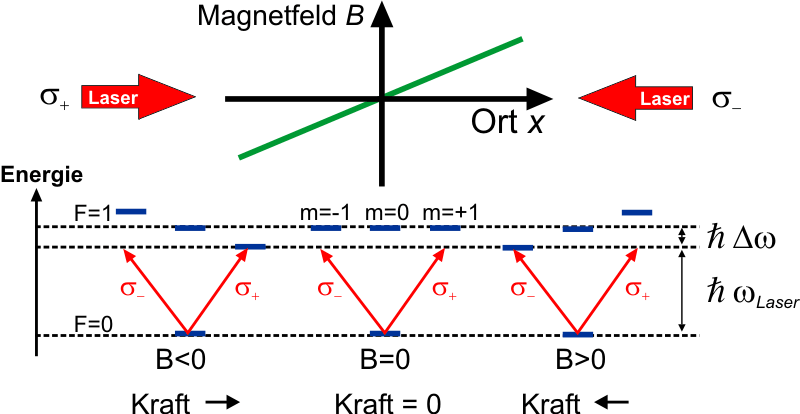
\includegraphics[width=0.7\textwidth]{Mot_posforce.png}
  \caption{die Aufspaltung des angeregten Zustands durch den Zeeman-Effekt und die ortsabhängige Kraft (Quelle: \url{https://de.wikipedia.org/wiki/Magneto-optische_Falle})}
  \label{zeemanmot}
  \end{figure}\\
 Damit begrenzt man die Atome räumlich. Während man die optische Melasse mit einer Reibungskraft vergleichen kann, wirkt die durch diese Anordnung erzeugte Kraft wie eine Federkraft. In drei Dimensionen erzeugt man ein Quadrupol-Magnetfeld durch Anti-Helmholtz-Spulen.
  \subsection{Übergänge von \ce{^{87} Rb}}
  In dem Versuch werden Rubidium-Atome verwendet. Rubidium ist zur Laserkühlung gut geeignet, da es Diodenlaser mit einer ähnlichen Frequenz wie der des Kühlübergangs von Rubidium gibt und das Element einen hohen Dampfdruck bei Raumtemperatur hat. Andere Atome muss man vorm Kühlen erhitzen, damit der Dampfdruck hoch genug ist um eine genügende Anzahl von Atomen in der Kammer zu haben. Das ist bei Rubidium allerdings nicht der Fall.
  
\ce{^{87} Rb} ist ein Alkalimetall, daher trägt nur das Elektron ($S=1/2$) in der äußersten Schale zum Drehimpuls $\vec{J}=\vec{L}+\vec{S}$ bei. Im Grundzustand $5S_{1/2}$ ($L=0$) besitzt das Atom also einen Drehimpuls $J = 1/2$. Der erste angeregten Zustand ist $5P_{3/2}$ ($L=1,\, J=3/2$). Der Kerndrehimpuls von \ce{^{87} Rb} ist $I=3/2$. Der Gesamtdrehimpuls $\vec{F}=\vec{I}+\vec{J}$ kann also im Grundzustand die Werte $F = 1$ und $F = 2$ annehmen. Im ersten angeregten Zustand sind $F'= 0,\, 1,\, 2,\, 3$ möglich. Das Termschema ist in Abbildung \ref{rb} zu sehen.

   Der Kühlübergang ist $\ket{F=2}\rightarrow\ket{F'=3}$. Es ist allerdings auch möglich, dass ein Atom von $\ket{F=2}$ nach $\ket{F'=2}$ angeregt wird. Von dort aus können die Atome in $\ket{F=2}$ (das stellt kein Problem dar) oder $\ket{F=1}$ fallen. Letztere kann der Kühllaser nicht mehr abbremsen. Daher gibt es noch einen Rückpumplaser um bei diesen Atomen wieder den Übergang $\ket{F=1}\rightarrow\ket{F'=2}$ anzuregen. Wenn sie von dort in den Zustand $\ket{F=2}$ fallen, können die Atome weiter gekühlt werden.
   \\Man benötigt also zwei Laser (Kühl- und Rückpumplaser), die leicht unterschiedliche Frequenzen haben. Der Frequenzabstand $\Delta$ ist dabei (Werte aus Abbildung \ref{rb}):
   \begin{align*}
     \omega_K & \approx - \SI{2,563}{\GHz} + \SI{384,230484}{\THz} + \SI{194}{\MHz} \\
     \omega_R & \approx \SI{4,272}{\GHz} + \SI{384,230484}{\THz} - \SI{73}{\MHz} \\
     \Delta & = \omega_R - \omega_K \\
     & \approx \SI{4,272}{\GHz} - \SI{73}{\MHz} + \SI{2,563}{\GHz} - \SI{194}{\MHz} \\
     & = \SI{6,568}{\GHz}
   \end{align*}
\newpage
  \begin{figure}[h!]
  \centering
  \includegraphics[page=10, width=\textwidth, trim=27mm 56mm 33mm 52mm, clip]{MOTDurchfuehrung.pdf}
  \caption{Termschema von \ce{^{87} Rb} (Kopie aus der Versuchsdurchführung)}
  \label{rb}
  \end{figure}
\newpage
\section{Bestandteile der MOT}
  \subsection{Die Laser}
    In dem Versuchsaufbau werden zwei Halbleiterlaser (Kühl- und Rückpumplaser)
    verwendet. Der Kühllaser wird mit ca. \SI{85}{\mA}, der Rückpumper mit ca.
    \SI{160}{\mA} betrieben. Durch Anlegen eines Stromes in Durchlassrichtung
    einer p-n-Diode entsteht eine dünne Schicht, in der es eine Besetzungsinversion
    mit Löchern im Valenz- und Elektronen im Leitungsband gibt. Als Resonator
    dienen die Stirnflächen der Diode. Durch Änderung des Stromes kann man die
    emittierte Wellenlänge ändern, allerdings erhöht sich gleichzeitig die
    Laserleistung. Ein Problem der Laser ist, dass sich durch leichte
    Temperaturänderungen die optische Weglänge des Lasers ändert und es somit zu
    Modensprüngen kommt. Um diese zu umgehen (und zum feineren Einstellen der
    Wellenlänge) wird ein Gitter als externe Cavity verwendet. Die erste
    Beugungsordnung wird dabei zurückreflektiert. Der Winkel, unter dem der Strahl
    von Gitter reflektiert wird ist von der Wellenlänge abhängig, daher kann man
    durch drehen des Gitters eine Änderung der Wellenlänge erreichen. Um das Gitter
    zu drehen ist es auf einem Piezo-Kristall befestigt. Durch Änderung des Stromes
    am Piezo-Element, ändert sich dessen Temperatur und damit dessen Ausdehnung, das
    Gitter wird also bewegt. Die Reflexion in die nullte Ordnung wird als Laserlicht
    verwendet. Um Rückreflexe in die Diode zu verhindern steht hinter den Lasern
    jeweils ein Isolator.
  \subsection{Die Sättigungsspektroskopie}
    Um die Laser zu koppeln wird ein kleiner Teil des Lichts in den
    Spektroskopiepfad ausgekoppelt. Dort befindet sich ein Aufbau zur
    Sättigungsspektroskopie. Dabei wird der Strahl durch eine Glasscheibe geschickt
    (es entstehen zwei Reflexe, einer an der Vorder- einer an der Rückseite der
    Scheibe) und über einen Spiegel in eine Rubidiumzelle geleitet (Pumpstrahl). Die
    beiden Reflexe von der Glasplatte werden ebenfalls in die Rubidiumzelle geschickt,
    allerdings von der anderen Seite (dadurch sind sie jeweils in die andere Richtung
    dopplerverschoben, wie der Pumpstrahl). Dabei passiert der stärkere Reflex
    (Abfragestrahl) in der Zelle einen Bereich, den auch der Pumpstrahl durchläuft.
    Beide brennen dadurch Löcher in das normale Dopplerprofil, die im gleichen
    Abstand links und rechts vom Maximum sind. Stellt man die Wellenlänge richtig ein,
    können sich beide Löcher im Profil überlagern (die Rubidiumatome können also von
    beiden Strahlen angeregt werden). Dies kann passieren, wenn man genau auf
    Resonanz mit einem Übergang ist (da beide Strahlen um den gleichen Betrag
    dopplerverschoben sind ist Absorption von Licht aus beiden Strahlen gleich
    wahrscheinlich $\rightarrow$ Lamb-Dip) oder wenn die Wellenlänge genau zwischen
    zwei Übergängen liegt (beide Strahlen regen jeweils unterschiedliche Übergänge an
    $\rightarrow$ Cross-Over-Resonanz). Da auf dem Oszilloskop die Absorption des
    Laserlichts angezeigt wird, erscheinen diese Dips als kleine Maxima im
    Dopplerprofil. Der schwächere Reflex von der Glasplatte durchläuft die
    Rubidiumzelle an einer anderen Stelle und misst somit zum Vergleich das reine
    Dopplerprofil.
    
    Um die Laser zu locken wird der Strom am Piezoelement so eingestellt, dass man
    genau den gewünschten Lamb-Dip erhält. Dabei wird auf dem Oszilloskop das
    Signal vom Abfragestrahl (mit Dopplerprofil) angezeigt, zum Locken wird die
    Differenz von Abfragestrahl und Dopplerprofil verwendet. Leichte Änderungen der
    Wellenlänge (z.B. durch wackeln der Cavity oder Temperaturänderungen) sorgen
    dafür, dass das Signal nicht mehr auf einem Maximum ist. Dann wird der Strom
    automatisch auf den richtigen Wert geregelt um wieder das Maximum zu erreichen.
    Da allerdings nicht klar ist, auf welcher Seite vom Maximum man sich befindet
    wird das Signal zunächst abgeleitet. Die Ableitung des Signals erfolgt durch
    Modulierung des Stromes mit einer Sinuskurve. Dies erlaubt Messungen auf beiden
    Seiten leicht neben dem betrachteten Punkt und somit eine Abschätzung der Steigung
    also eine Ableitung. Das Locken erfolgt dann auf einem Nulldurchgang der Ableitung.
  \subsection{Der Akusto-optische Modulator}
    Das Locken des Kühllasers erfolgt auf die Cross-Over-Resonanz der Übergänge
    $\ket{F=2}\rightarrow\ket{F'=1}$ und $\ket{F=2}\rightarrow\ket{F'=3}$:
    \begin{align*}
      \omega_{co} &=
      -\SI{2.563}{\GHz} + \SI{384.230484}{\THz} + (\SI{193}{\MHz} - \SI{229}{\MHz})/2\\
      &= \SI{384.227903}{\THz}
    \end{align*}
    Der Übergang, den der Kühllaser jedoch anregen soll ist
    $\ket{F=2}\rightarrow\ket{F'=3}$:
    \begin{align*}
      \omega_{K} &= -\SI{2.563}{\GHz} + \SI{384.230484}{\THz} + \SI{193}{\MHz}\\
      &= \omega_{co} + (\SI{193}{\MHz} + \SI{229}{\MHz})/2\\
      &= \omega_{co} + \SI{211}{\MHz}
    \end{align*}
    Um die Differenz auszugleichen wird ein akusto-optischer Modulator (AOM)
    verwendet. Im AOM ist eine Bragg-Zelle, in der eine Schallwelle erzeugt wird. Durch
    diese Schallwelle ändert sich der Brechungsindex in der Zell periodisch. Daher
    wirkt die Bragg-Zelle wie ein Gitter, es werden also mehrere Beugungsordnungen mit
    je nach Ordnung geänderten Wellenlängen reflektiert. Hier wird die erste Ordnung
    durch eine Blende isoliert. Dieser Strahl hat eine höhere Frequenz, als der
    Einlaufende. Wie groß die Frequenzänderung ist hängt von der Spannung am AOM ab und
    kann einer Eichkurve in der Anleitung entnommen werden. Danach wird die erste
    Ordnung in den AOM zurückreflektiert (AOM-Doppelpass). Dies bewirkt eine erneute
    Frequenzerhöhung, man muss also die doppelte AOM-Frequenz addieren um die Frequenz
    des Strahls nach dem Doppelpass zu erhalten. Mit der Eichkurve ergibt sich eine
    optimale Spannung am AOM von \SI{18.5}{\V} (um den Übergang genau zu treffen, für
    die MOT ist allerdings eine leicht verschobene Frequenz nötig).
  \subsection{Der Trapezverstärker}
    Nachdem die Strahlen des Kühl- und des Rückpumplasers überlagert werden durchlaufen
    sie um die Leistung zu erhöhen einen Trapezverstärker (engl. tapered amplifier
    (TA)). Ein TA besteht im wesentlichen aus einem aktiven Medium (hier eine
    p-n-Diode), wie bei einem Laser. Auch bei einem TA wird durch Pumpen (hier durch
    Ströme von ca. \SI{1}{\A}) eine Besetzungsinversion erzeugt. Allerdings fehlt ein
    optischer Resonator um von spontaner zu stimulierter Emission überzugehen.
    Stattdessen wird ein Laserstrahl (Seed) eingekoppelt, der Übergänge anregt. Als
    Resultat erhält man einen Strahl mit wesentlich höherer Leitung (siehe Abschnitt
    \ref{intensities}). Um im Trapezverstärker genügend stimulierte Emission anzuregen
    muss der Laserstrahl den TA möglichst genau durchlaufen. Dies erreicht man durch
    ein Spiegelpaar vor dem TA, mit dem man Strahlrichtung und -lage anpassen kann. Das
    justieren erfolgt bei niedrigen Strömen, da das Betreiben eines Trapezverstärkers
    ohne Seed der Diode schadet. Wie bei den Lasern steht auch hinter dem TA ein
    Isolator um Rückreflexe zu vermeiden. Danach wird der Strahl durch eine Glasfaser
    zum Aufbau der eigentlichen MOT geleitet.
  \subsection{Die Vakuumkammer}
    Die Vakuumapparatur war im Versuch bereits aufgebaut und in Betrieb, man musste nur
    jeweils zum erzeugen einer MOT Rubidium in die Kammer bringen. Dies geschah mittels
    Dispensern, die durch Ströme von ca. \SI{3}{\A} zum Glühen gebracht wurden und
    dadurch Rubidium-Dampf abgaben. Dabei musste man darauf achten, dass die Dispenser
    nicht zu lange am Stück liefen und der Druck in der Vakuumkammer nicht zu groß
    wurde, da die Dispenser sonst schnell leer werden könnten und ersetzt werden
    müssten. Daher mussten die Zeit und der Strom an den Dispensern, sowie der Druck in
    der Kammer in ein Laborbuch eingetragen werden.
  \subsection{Die Kamera}
    Es stehen im Versuch zwei Kameras zur Verfügung. Eine Fingerkamera für qualitative
    Beobachtungen (da sie eine automatische Helligkeitsregelung hat) und eine
    CCD-Kamera für quantitative Messungen. Die CCD-Kamera musste zunächst geeicht
    werden (siehe Abschnitt \ref{eichung}). Mit der CCD-Kamera sollte die Atomzahl in
    der MOT bestimmt werden, aus der Eichung konnte die Photonenanzahl pro Pixel
    berechnet werden. Daher ist es noch notwendig die Anzahl von Photonen, die ein Atom
    emittiert zu bestimmen. Der Teil des Lichts, der von der Kamera aufgenommen wird
    ist (mit Abstand $a = \SI{28}{\cm}$ zum Objektiv und Objektivdurchmesser $d =
    \SI{4.5}{\cm}$):
    \begin{align*}
      \alpha = \frac{4 \pi (d / 2)^2}{\pi a^2} = \SI{2.58}{\percent}
    \end{align*}
    Ein Anteil $\beta$ von ca. \SI{4}{\percent} geht durch Reflexionen verloren. Die
    gesamte von der Atomwolke emittierte Leistung $P_{ges}$ ergibt sich also bei einer
    von der Kamera gemessenen Leistung von $P_{gem}$ aus:
    \begin{align*}
      P_{ges} = \frac{P_{gem}}{\alpha (1 - \beta)} = 40.33 P_{gem}
    \end{align*}
    Die gemessene Leistung ist gegeben durch
    \begin{align*}
      P_{gem} &= \frac{n \hbar \omega}{t} \\
      &= \frac{\hbar \omega}{t} \frac{\text{Photonen}}{\text{Count}} \text{Counts}
    \end{align*}
    mit der Anzahl $n$ von Photonen, die die Kamera registriert, Licht der Energie
    $\hbar \omega$, der Belichtungszeit $t = \SI{19.932}{\ms}$ der Kamera und dem
    Umrechnungsfaktor $\frac{\text{Photonen}}{\text{Count}}$ aus Abschnitt
    \ref{eichung}.
    Die Leistung $P_A$, die ein Atom abstrahlt ist (mit der Streurate $1 / \tau_z$):
    \begin{align*}
      P_A = \frac{\hbar \omega}{\tau_z}
    \end{align*}
    Die Anzahl $N$ der Atome in der Falle ist das Verhältnis der abgestrahlten Leistung
    aller Atome zur Leistung des Lichts eines Atoms:
    \begin{align*}
      N &= \frac{P_{ges}}{P_A} \\
      &= \frac{1}{\alpha (1 - \beta)} \frac{\tau_z}{t}
        \frac{\text{Photonen}}{\text{Count}} \text{Counts}
    \end{align*}
    Die Streurate ist:
    \begin{align*}
      \tau_z = \left(
        \frac{\Gamma}{2}
        \frac{I_{ges} / I_0}{1 + I_{ges} / I_0 + (2 \delta / \Gamma)^2}
      \right)^{-1}
    \end{align*}
    Dabei ist die Sättigungsintensität $I_0 = \SI{16}{\W\per\square\m}$, die
    Linienbreite $\Gamma = 2 \pi \cdot \SI{6}{\MHz}$ und die Intensität des Laserlichts
    $I_{ges} = \SI{87.7}{\mega\W\per\square\m}$. Die Frequenzverschiebung $\delta$ ist
    (bei einer Spannung von \SI{20}{\V} am AOM):
    \begin{align*}
      \delta = (\omega_{co} + 2 \omega_{AOM}) - \omega_K = \SI{55.78}{\MHz}
    \end{align*}
    Mit diesen Werten ergibt sich $\tau_z = \SI{53}{\nano\s}$. Mit
    $\frac{\text{Photonen}}{\text{Count}} = 4869.2$ erhält man:
    \begin{align*}
      N = 0.5 \text{Counts}
    \end{align*}
    Mit diesem Umrechnungsfaktor, sowie dem Abbildungsmaßstab ist es möglich Atomzahl
    und Größe einer Atomwolke in der MOT zu bestimmen.
\newpage
\section{Messungen}
  \subsection{Intensitätsmessungen im Strahlengang}
    \label{intensities}
  Am Anfang des Versuchs haben wir geprüft, ob alle optischen Komponenten richtig justiert sind. Dazu haben wir mit dem Leistungsmesskopf (Laserdiode) die Lichtleistungen an der geforderten Stellen (wie man in Abbildung \ref{leistung} sehen kann) gemessen. Dabei waren  Rückpump- bzw. Kühllaser mit \SI{164,0}{\mA} bzw. \SI{86,1}{\mA} im Betrieb. Von der Ausgangsleistung geht jeweils ein Teil in den Isolatoren verloren (beim Rückpumper mit \SI{5,3}{\mW} relativ viel, was allerdings nicht schlimm ist, da das Signal des Rückpumpers in der MOT nicht stark sein muss). Ein kleiner Teil wird in den Spektroskopiepfad ausgekoppelt (\SI{0,7}{\mW} bzw. \SI{0,5}{\mW}). Da im AOM-Doppelpass einige Ordnungen ausgeblendet werden, ist die Leistung des Kühllasers danach um \SI{9,8}{\mW} geringer. Nachdem die Strahlen von Kühl- und Rückpumplaser überlagert werden, bringt ein $\lambda /2$-Plättchen sie auf die gleiche Polarisation. Dabei geht wieder Leistung verloren. Vor dem TA sind noch \SI{4,8}{\mW} übrig.
    \begin{figure}[h!]
  \centering
  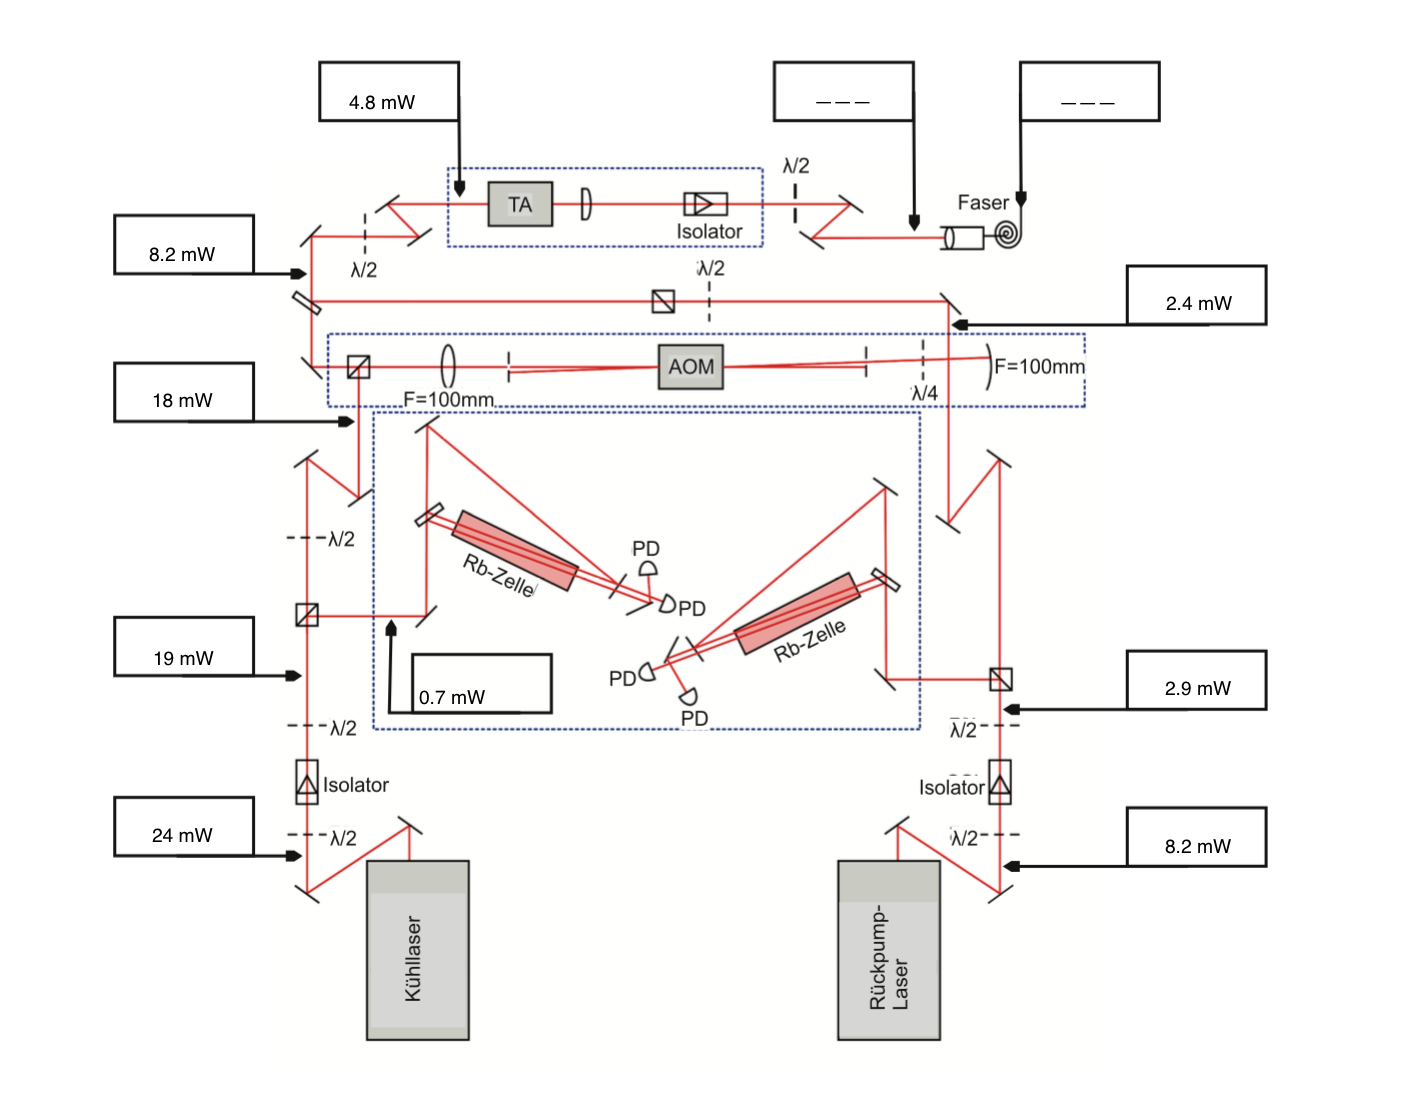
\includegraphics[width=\textwidth]{Strahlenleistungen.png}
  \caption{gemessenen Leistungen im Lasersystem}
  \label{leistung}
  \end{figure}
\\Wir haben auch die Strahlleistung vor der Faser für zugehörige Ströme am TA gemessen, die Werte sind in Tabelle \ref{tatab} zu sehen. Je größer der Strom am TA ist, desto mehr angeregte Zustände gibt es im TA. Der Zusammenhang scheint exponentiell zu sein (siehe Abbildung \ref{TA}). Für größere Ströme ist eine Sättigung zu erwarten, da irgendwann nicht mehr Löcher ins Leitungsband gelangen können. Durch die Faser kamen in der Regel ca. $30\%$ der Leistung.
\begin{figure}[h!]
\centering
 \begin{tabular}{|c|c|}\hline
 TA Strom in \si{\mA}&Strahlleistung vor Faser in \si{\mW}\\ \hline \hline
400&2.3\\ \hline
500&5.4\\ \hline
600&12.5\\ \hline
700&25.5\\ \hline
800&49\\ \hline
900& Ende d. Skala\\ \hline
\end{tabular}
\caption{Leistung des verstärkten Strahls für verschiedene Ströme am TA}
\label{tatab}
\end{figure}
    \begin{figure}[h!]
  \centering
  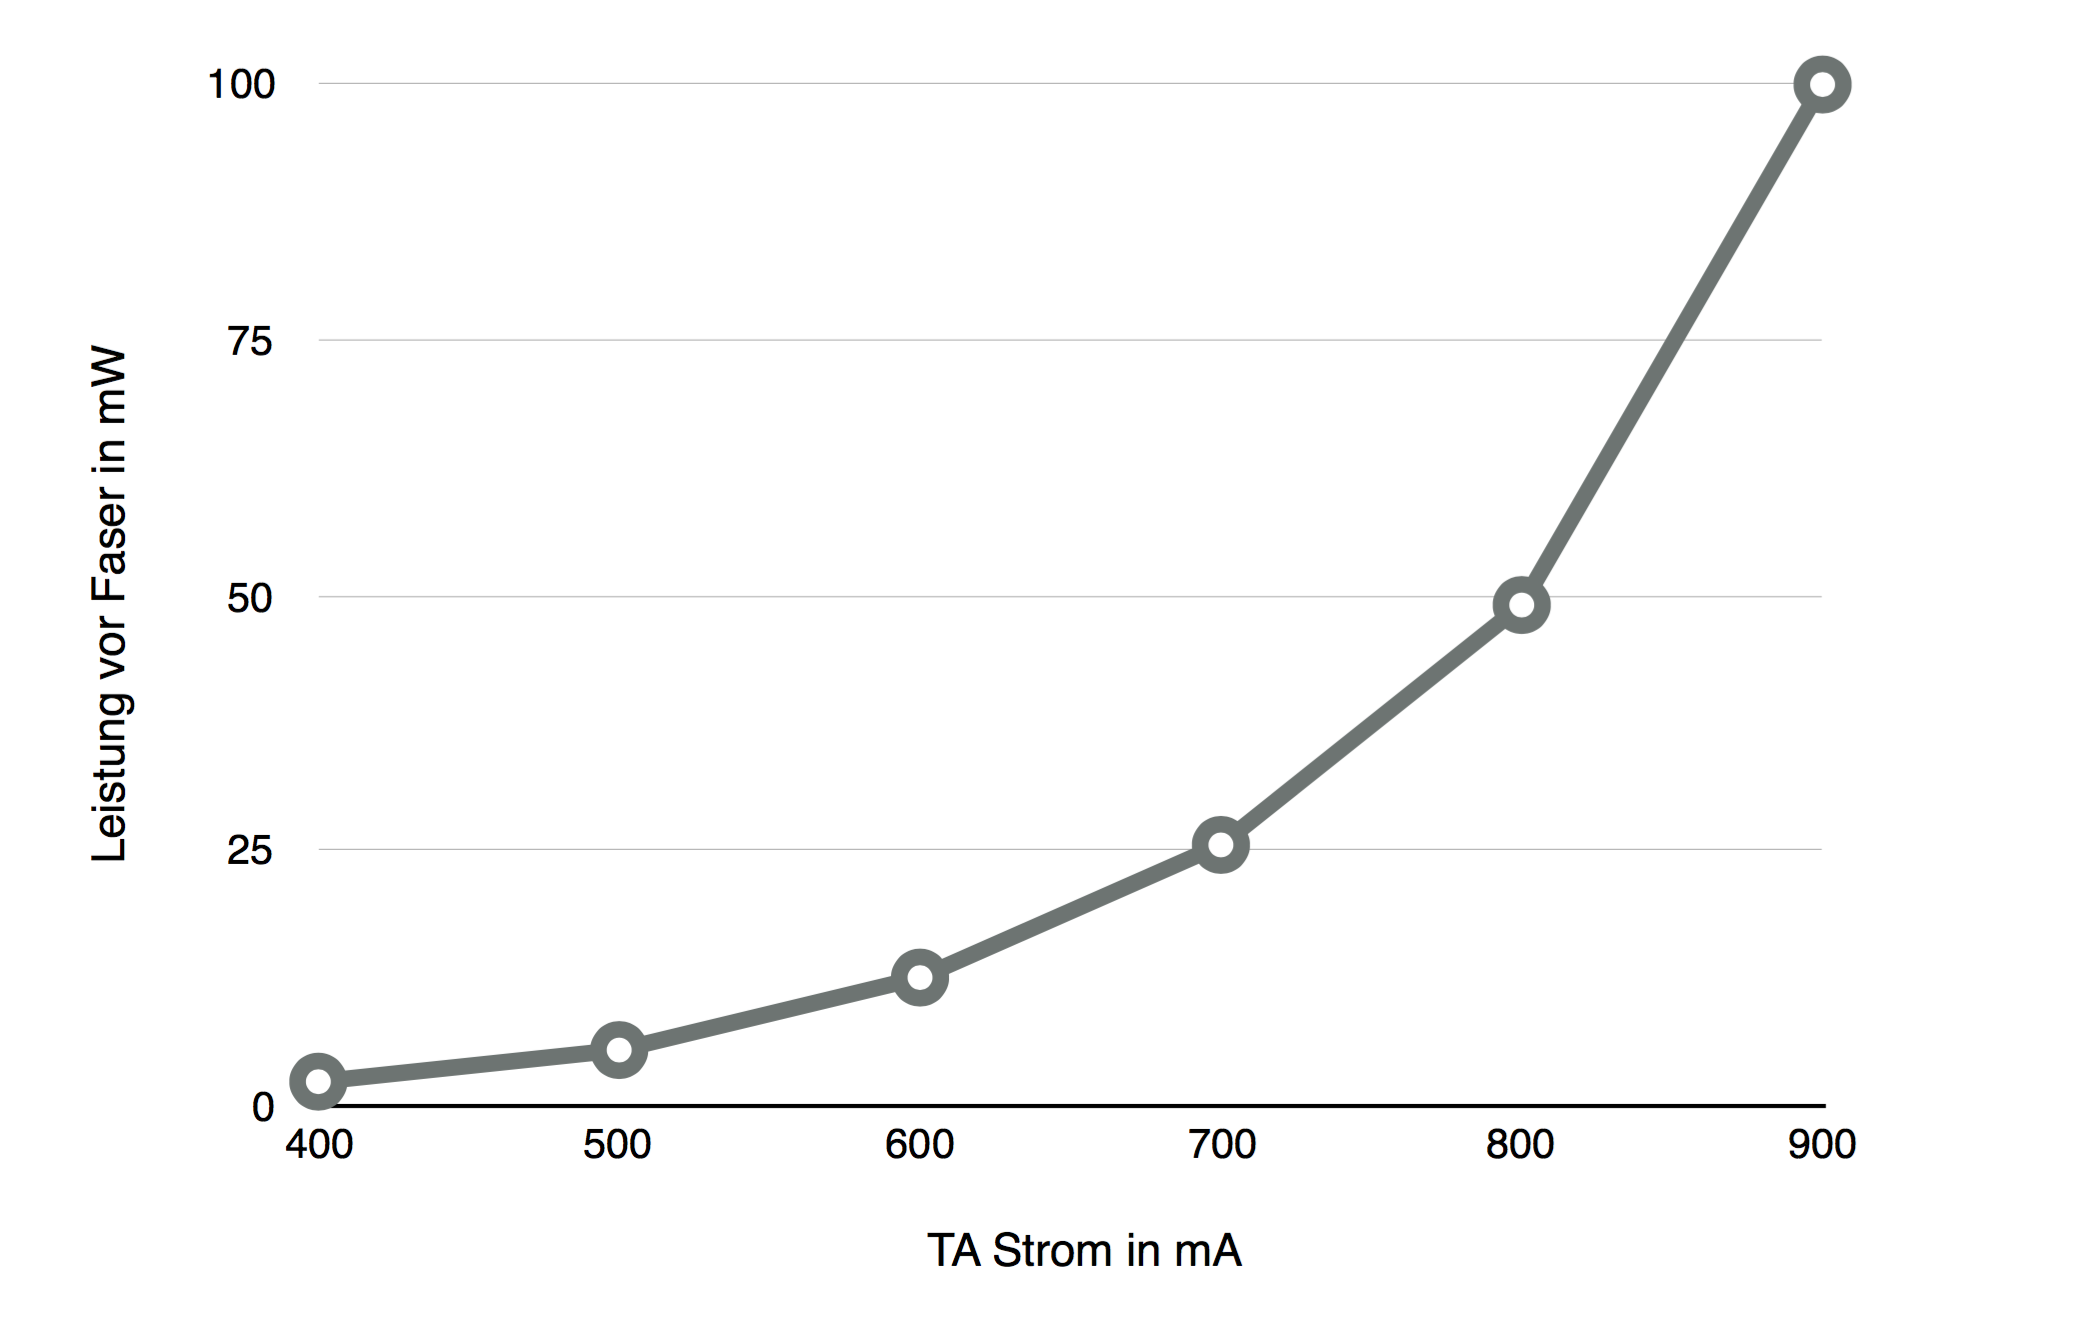
\includegraphics[width=0.7\textwidth]{TA.png}
  \caption{Zugehörige Diagramm}
  \label{TA}
  \end{figure}
  \subsection{Vermessung der Strahlbreite}
 Um die Anzahl von Teilchen in der MOT zu berechnen, ist es wichtig die Intensität des Laserstrahls zu kennen. Da wir nur die Leistung vom Strahl messen konnten, war es erforderlich, den Strahldurchmesser zu bestimmen.\\
 Dazu haben wir eine Klinge, die mit einer Mikrometerschraube bewegbar war, in horizontaler und vertikaler Richtung so in den Strahl geschoben, dass man jeweils 70 und 30 Prozent der Leistung vom Strahl messen konnte. Daher haben wir die unteren $x$ Werte (die Stellung der Schraube). Diese Werte kann man in die folgende Formel einsetzen, um den waist (engl. für Strahlbreite) $\omega_h$ und $\omega_v$ auszurechnen:
  \begin{align*}
  \omega_h & \approx 2.828(x_{70\%}-x_{30\%})
  =2.828(6.43-4.21) \si{\micro\m}\\
  &=\SI{6.278}{\micro\m}\\
  \omega_v &\approx 2.828(x_{70\%}-x_{30\%})=2.828(2.63-4.67) \si{\micro\m}\\&=\SI{5.769}{\micro\m}
   \end{align*}
   Damit können wir jetzt die Strahlfläche $F$ ausrechnen:
   \begin{align*}
   F=\pi \omega_h \omega_v =\SI{113.806}{\micro\m^2}
   \end{align*}
   Und jetzt können wir die Intensität $I$ ausrechnen, wobei die Leistung vom Strahl ohne Klinge \SI{10} {\mW} ist:
   \begin{align*}
   I=\frac{P}{F}=\frac{\SI{e-2}{\W}}{\SI{113.806e-12}{\m^2}}=\SI{87.7}{\mega\W\per\square\m}
   \end{align*}
  \subsection{Eichung der Kamera}
  \label{eichung}
  Wir haben erstmal mit Millimeterpapier gemessen, wieviele Pixel der Kamera einem Quadratmeter entsprechen. Dabei haben wir Millimeterpapier im gleichen Abstand wie zur MOT angebracht und dann mit dem Kameraprogramm ein Foto gemacht. Wir haben ein Kästchen von \SI{1}{\cm^2} davon ausgewählt und mit Mathematica (wie in der Durchführung erklärt) die Anzahl der Pixel bestimmt. Pixel in x-Richtung: $256$. Pixel in y-Richtung: $258$. Mit dem Mittelwert der beiden Zahlen ($257$) haben wir den Skalierungsfaktor \SI{38.9105}{\micro\m\per Pixel} berechnet.\\
  Danach haben wir zwei Fotos gemacht, einmal ohne Laserstrahl (nur Hintergrund) und einmal mit dem Laserstrahl direkt auf die Kamera gerichtet. Dazu haben wir einen Filter benutzt um das Licht abzuschwächen und eine Linse damit der Strahl nicht fokussiert ist. Sonst hätte es Bereiche gegeben, in denen die Kamera sättigt. Die Anzahl der Counts wurde vom Kameraprogramm angezeigt. Dadurch kann man weiter den Eichfaktor Photonen Pro Count ausrechnen. Die Leistung des eingestrahlten Lichts ist das Produkt aus der Energie der Photonen ($n\hbar\omega$ bei $n$ Photonen) und der Belichtungszeit $t=\SI{19.932}{\mm}$. Andererseits haben wir die Leistung vor dem Filter (optische Dichte 3) gemessen. Also ist:
  \begin{align*}
  \lambda &=\SI{780.246}{\nano\m},\, t=\SI{19.932}{\milli\m},\, \text{OD}=3,\, P=\SI{1.404}{\milli\W},\, E=\frac{h c}{\lambda} \\
  n \frac{h c}{\lambda}&=P 10^{-\text{OD}} \\
  \Rightarrow \frac{\text{Photonen}}{\text{Counts}} &=4869.2
  \end{align*}
\end{document}